\documentclass{thesis_massaro}

\makeatletter

\newenvironment{formatparttext}{}

% Pour une raison que j'ignore, malgre le [frenchb]{babel}
% les noms sont en anglais
\renewcommand{\chaptername}{Chapitre}
\renewcommand{\contentsname}{Table des Mati\`eres}
\renewcommand{\bibname}{Bibliographie}
\renewcommand{\tablename}{Tableau}
\renewcommand{\listfigurename}{Liste des Figures}

\lstset{language=C,captionpos=b,frame=single}
\def\listingsfont{\ttfamily}

\newtheorem{theorem}{Théorème}[section]
\newtheorem{prop}{Propriété}[section]
\newtheorem{propo}{Proposition}[section]
\newtheorem{lemma}{Lemme}[section]
\newtheorem{definition}{Définition}[section]

\newcommand{\parttext}[1]{\def\@parttext{#1}}
\def\@endpart{\vskip 0pt plus 0.5fil
    \begin{formatparttext}
        \@parttext
        \gdef\@parttext{}
    \end{formatparttext}
    \vskip 0pt plus 0.5fil
    \newpage
    \if@twoside
    \if@openright
    \null
    \thispagestyle{empty}%
    \newpage
    \fi
    \fi
    \if@tempswa
    \twocolumn
\fi}
\makeatother

\def\blurb{%
    Nom établissement d'acceuil \\
    adresse établissement d'acceuil\\
    XXXX Ville
}

\def\clap#1{\hbox to 0pt{\hss #1\hss}}%

\def\ligne#1{%
    \hbox to \hsize{%
\vbox{\centering #1}}}%

\def\haut#1#2#3{%
    \hbox to \hsize{%
        \rlap{\vtop{\raggedright #1}}%
        \hss
        \clap{\vtop{\centering #2}}%
        \hss
\llap{\vtop{\raggedleft #3}}}}%

\def\bas#1#2#3{%
    \hbox to \hsize{%
        \rlap{\vbox{\raggedright #1}}%
        \hss
        \clap{\vbox{\centering #2}}%
        \hss
\llap{\vbox{\raggedleft #3}}}}%


\let \oldref \ref
\renewcommand{\ref}[1]{(\oldref{#1})}

% Mise en page
% Indentation paragraphe
\setlength{\parindent}{0pt}
\setlength{\parskip}{12pt}


\renewcommand{\nomgroup}[1]{%
  \ifthenelse{\equal{#1}{B}}{%
    \item[]\hspace*{-\leftmargin}%
    \rule[2pt]{0.45\linewidth}{1pt}%
    \hfill \textbf{Chapitre 1} \hfill
    \rule[2pt]{0.45\linewidth}{1pt}
  }{%

    \ifthenelse{\equal{#1}{C}}{%
      \item[]\hspace*{-\leftmargin}%
      \rule[2pt]{0.45\linewidth}{1pt}%
      \hfill \textbf{Chapitre 2} \hfill
      \rule[2pt]{0.45\linewidth}{1pt}
    }{}
  }
}


%\newtoggle{remake}

%%% Local Variables:
%%% mode: latex
%%% TeX-master: "these_michel"
%%% End:


\begin{document}

%\toggletrue{remake}
%\togglefalse{remake}

\dominitoc
\pagenumbering{roman}

\newpage

%Pour avoir la version officielle de la fac
%\includepdf[pages= 1]{Couverture/Couv.pdf} %Insérer la première page

%\newpage
%\thispagestyle{empty}
%\null
%\newpage
%\thispagestyle{empty}
%\null
%\newpage
%\thispagestyle{empty}
%\null
%\newpage


\newgeometry{margin=0.45in}
\thispagestyle{empty}\vbox to .9\vsize{

    \vss
    \vbox to 1\vsize{

        \vspace{2cm}      

        \haut{}{\blurb}{}
        \vspace{1.5cm}
        \vfill
        \ligne{\LARGE{\textbf{\textsc{TH\`ESE DE DOCTORAT \\ DE L'UNIVERSIT\'E
                DE XXXXXXXXX}}}}
        \vspace{3mm}
        \ligne{\large{\textbf{\textsc{\'Ecole Doctorale de Nom de l'école,
                \\ doctorale}}}} 
        \vspace{3mm}
        \ligne{\textit{Spécialité}}
        \vspace{3mm}
        \ligne{\large{\textbf{\textsc{Nom Spécialité}}}}
        \vspace{3mm}
        \ligne{\textit{Présentée par}}
        \vspace{3mm}
        \ligne{\textbf{\large{Prenom \textsc{Nom}}}}
        \vspace{3mm}
        \ligne{\textit{Pour obtenir le grade de}}
        \vspace{3mm}
        \ligne{\textbf{\large{DOCTEUR DE L'UNIVERSIT\'E DE XXXXXX}}}

        \vspace{1.8cm}
        \ligne{\huge{\textbf{\textsc{Titre de la thèse}}}}
        \vspace{1.8cm}
        \vfill
        \ligne{
            \begin{tabular}{l}
                \textit{Soutenue le} XX XXXX XXXX \textit{devant le jury composé de} :
        \end{tabular}}
        \vspace{5mm}
        \ligne{
            \begin{tabular}{rll}
              \hline \\
             \textit{Rapporteur} : & Prénom Nom & \textit{Etablissement}\\
             \textit{Rapporteur} : & Prénom Nom & \textit{Etablissement}\\
             \textit{Directeur de thèse} : & Prénom Nom &
                                             \textit{Etablissement}\\
             \textit{Examinateur} : & Prénom Nom &
                                            \textit{Etablissement}\\ 
             \textit{Examinateur} : & Prénom Nom &
                                            \textit{Etablissement}\\ 
             \textit{Examinateur} : & Prénom Nom & 
                                      \textit{Etablissement}\\
              \hline
            \end{tabular}
        }
        \vspace{1.8cm}
    }
    \vss
}
\restoregeometry


\newpage
\thispagestyle{empty}
\null

\chapter*{Remerciements}
\markboth{\MakeUppercase{Remerciements}}{\MakeUppercase{Remerciements}}
\addstarredchapter{Remerciements}

\lipsum[4-5]


\cleardoublepage
\thispagestyle{empty}
\tikzsetnextfilename{generated_figures/dedication}
\begin{tikzpicture}
  \node[white] at (0,0) {none.};
  \node at (12,-4) {\textit{Dedication.}};
\end{tikzpicture}


\newpage
\thispagestyle{empty}
\null
\newpage

\makenomenclature

\begin{spacing}{0.1}
\tableofcontents
\listoffigures


\end{spacing}

\cleardoublepage
\markboth{\MakeUppercase{Liste des symboles}}{\MakeUppercase{Liste des symboles}}
\printnomenclature[3cm]



\cleardoublepage
\pagenumbering{arabic}

\chapter*{Introduction}
\markboth{\MakeUppercase{Introduction}}{\MakeUppercase{Introduction}}
\addstarredchapter{Introduction}

\lipsum[4-5]


\chapter{Titre}
\label{chap:lab1}

\epigraph{The most exciting phrase to hear in science, the one that heralds new
  discoveries, is not "Eureka!" (I found it!) but rather, "hmm.... that's
  funny..."}{Isaac Asimov}

\minitoc % Sommaire du chapitre


\section[Titre dans le sommaire]{Titre}

\lipsum[1-1]

$$\sum_i x^i y^i$$

\lipsum[2-2]

\begin{figure}[H]
  \centering

  \tikzsetnextfilename{generated_figures/figure-exemple} 
  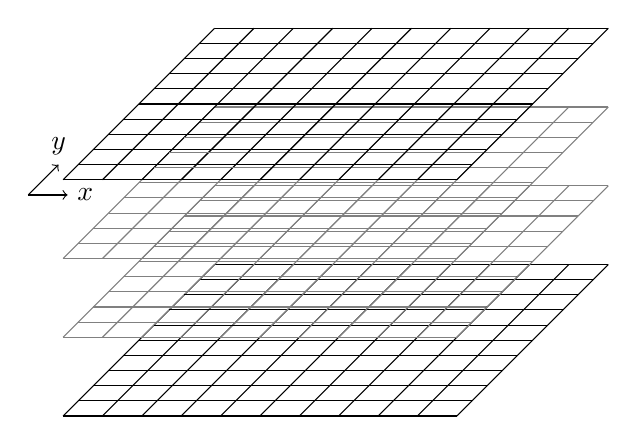
\begin{tikzpicture}[scale=0.5]
  \draw[->] (-0.5,6,11) -- (0.5,6,11);
  \draw[->] (-0.5,6,11) -- (-0.5,6,9);

  \draw (0.5,6,11) node[anchor=west] {$x$};
  \draw (-0.5,6,9) node[anchor=south] {$y$};

  \foreach \i in {0,...,10}{
    \draw (\i,6,0) -- (\i,6,10);
    \draw (0,6,\i) -- (10,6,\i);

    \draw[draw=gray] (\i,4,0) -- (\i,4,10);
    \draw[draw=gray] (0,4,\i) -- (10,4,\i);

    \draw[draw=gray] (\i,2,0) -- (\i,2,10);
    \draw[draw=gray] (0,2,\i) -- (10,2,\i);

    \draw (\i,0,0) -- (\i,0,10);
    \draw (0,0,\i) -- (10,0,\i);
  }
\end{tikzpicture}


  \caption{Légende.}
  \label{fig:tag}
\end{figure}

\subsection{Titre}

\lipsum[3-3]



\nomenclature[b01]{$x$}{Définition 1.}
\nomenclature[b02]{$y$}{Définition 2.}

\chapter{Titre}
\label{chap:lab2}

\epigraph{To err is human, but to really foul things up you need a
  computer}{Paul R. Ehrlich}

\minitoc % Sommaire du chapitre


\section[Titre dans le sommaire]{Titre}

\lipsum[1-1]

$$\sum_i z^i$$

\lipsum[2-2]

\subsection{Titre}

\lipsum[3-3]



\nomenclature[c01]{$z$}{Définition 3.}

\chapter*{Conclusion}
\markboth{\MakeUppercase{Conclusion}}{\MakeUppercase{Conclusion}}
\addstarredchapter{Conclusion}

\lipsum[4-5]


\renewcommand{\thechapter}{\Alph{chapter}}

\setcounter{chapter}{0}

\chapter{Titre}\label{sec:Annexe}

\lipsum[2-4]





\cleardoublepage
\phantomsection
\addcontentsline{toc}{chapter}{Bibliographie}
\nocite{*}
\bibliographystyle{plain}
\bibliography{references}

%\newpage
%\thispagestyle{empty}
%\null
%\newpage
%\thispagestyle{empty}
%\null
%\newpage
%\thispagestyle{empty}
%\null
%\newpage
%\thispagestyle{empty}
%\null
%\newpage

%\cleardoublepage
%Pour inclure la dernière page, page officielle de la fac
%\setcounter{page}{0}
%\includepdf[page= 2]{Couverture/Couv.pdf}%Insérer la première page


\end{document}
